% Source: AESP_466_ClassWork/Assignments/Assignment_3/textbook_example_problems/E6.2/wing_planform_tikz.tex
\documentclass[tikz,border=8pt]{standalone}
\usetikzlibrary{arrows.meta,calc}

% USC Brand Colors
\definecolor{USCGarnet}{HTML}{73000A}
\definecolor{USCAtlantic}{HTML}{466A9F}
\definecolor{USCHorseshoe}{HTML}{65780B}  % Green from brand palette
\definecolor{USCBlack}{HTML}{000000}

\begin{document}
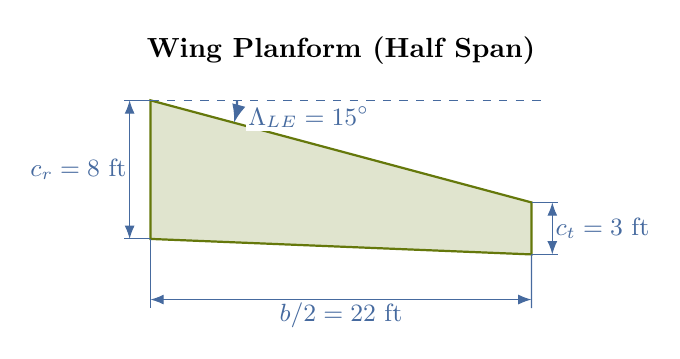
\begin{tikzpicture}[>=Latex,line cap=butt,line join=miter]

% Scale for display
\def\scale{0.22}

% Wing geometry - longer span, less sweep for transport aircraft
\def\rootchord{8}        % root chord (ft)
\def\tipchord{3}         % tip chord (ft)
\def\semispan{22}        % half wingspan (ft) - longer span
\def\sweepangle{15}      % leading edge sweep (degrees) - less sweep
\pgfmathsetmacro{\tipoffset}{\semispan * tan(\sweepangle)}  % LE sweep offset

\begin{scope}[scale=\scale]

% Wing coordinates (half-span view)
% y = spanwise (horizontal), x = chordwise (vertical, down is aft)
\coordinate (RootLE) at (0,0);
\coordinate (RootTE) at (0,-\rootchord);
\coordinate (TipLE) at (\semispan,-\tipoffset);
\coordinate (TipTE) at (\semispan,-\tipoffset-\tipchord);

% Fill wing
\fill[USCHorseshoe!20] (RootLE) -- (TipLE) -- (TipTE) -- (RootTE) -- cycle;

% Wing outline
\draw[USCHorseshoe,thick] (RootLE) -- (TipLE) -- (TipTE) -- (RootTE) -- cycle;


% ---- DIMENSIONS ----

% Root chord dimension (left side)
\draw[USCAtlantic,thin] (RootLE) -- ++(-1.5,0);
\draw[USCAtlantic,thin] (RootTE) -- ++(-1.5,0);
\draw[<->,USCAtlantic] (-1.2,0) -- (-1.2,-\rootchord)
    node[midway,left,fill=white,inner sep=1pt,font=\small] {$c_r = \rootchord$ ft};

% Tip chord dimension (right side)
\draw[USCAtlantic,thin] (TipLE) -- ++(1.5,0);
\draw[USCAtlantic,thin] (TipTE) -- ++(1.5,0);
\draw[<->,USCAtlantic] (\semispan+1.2,-\tipoffset) -- (\semispan+1.2,-\tipoffset-\tipchord)
    node[midway,right,fill=white,inner sep=1pt,font=\small] {$c_t = \tipchord$ ft};

% Semispan dimension (bottom)
\draw[USCAtlantic,thin] (RootTE) -- (0,-\rootchord-4);
\draw[USCAtlantic,thin] (TipTE) -- (\semispan,-\rootchord-4);
\draw[<->,USCAtlantic] (0,-\rootchord-3.5) -- (\semispan,-\rootchord-3.5)
    node[midway,below,fill=white,inner sep=1pt,font=\small] {$b/2 = \semispan$ ft};

% ---- SWEEP ANGLE ----
% Reference line (spanwise direction from root LE)
\draw[USCAtlantic,dashed,thin] (RootLE) -- (\semispan+1,0);

% Sweep angle arc
\draw[USCAtlantic,thick,->] (5,0) arc[start angle=0, end angle=-\sweepangle, radius=5]
    node[pos=0.5,right,xshift=3pt,yshift=-2pt,fill=white,inner sep=1pt,font=\small] {$\Lambda_{LE} = \sweepangle^\circ$};

% Title
\node[above,font=\bfseries] at (\semispan/2,1.5) {Wing Planform (Half Span)};

\end{scope}

\end{tikzpicture}
\end{document}
